\begin{landscape}

\begin{tabular}{p{2in}p{2in}p{2in}p{2in}}
\centering
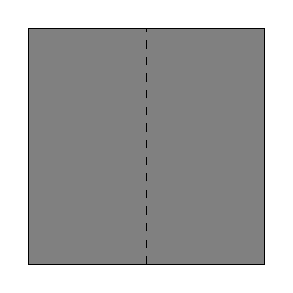
\begin{tikzpicture}[scale=.75]
	\draw[fill=gray] (0,0) rectangle (4,4);
	\draw[dashed] (2,0) -- (2,4);
\end{tikzpicture}

Fold paper in half 
	& 
{\centering
	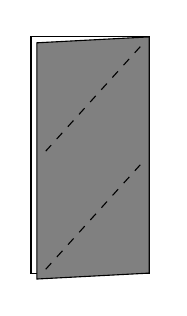
\begin{tikzpicture}[scale=.75]
		\draw (0,0) rectangle (2,4);
		\draw[fill=gray] (.1,-.1) node (A) {} -- (2,0) -- (2,4) node[pos=.5] (B) {} node (C) {}-- (.1,3.9)  -- cycle node[pos=.5] (D) {};
		\draw[dashed] (A) -- (B);
		\draw[dashed] (C) -- (D);
	\end{tikzpicture}}
	
Bring one corner to opposite edge to form a triangle and repeat with opposite corner	
	& 
\centering	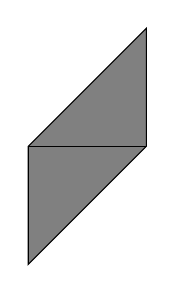
\begin{tikzpicture}[scale=.75]
		\draw[fill=gray] (0,0) -- (2,2) -- (2,4) -- (0,2) --cycle;
		\draw (0,2) -- (2,2);
	\end{tikzpicture}
	
	You should see a parallelogram
	& 
	\centering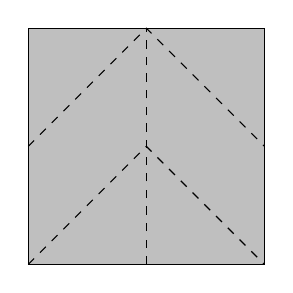
\begin{tikzpicture}[scale=.75]
	\draw[fill=lightgray] (0,0) rectangle (4,4);
	\draw[dashed] (2,0) -- (2,4);
		\draw[dashed] (0,0) -- (2,2) -- (4,0);
		\draw[dashed] (0,2) -- (2,4) -- (4,2);
\end{tikzpicture}

Open the paper
	\end{tabular}
	
	\begin{tabular}{p{2in}p{2in}p{2in}p{2in}}

	
	{\centering 
	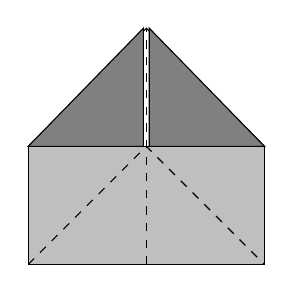
\begin{tikzpicture}[scale=.75]
	\begin{scope}
			\draw[fill=lightgray] (0,0) rectangle (4,2);
	\draw (0,2) -- (2,4) -- (4,2);
	\draw[dashed] (2,0) -- (2,4);
		\draw[dashed] (0,0) -- (2,2) -- (4,0);
		\draw[fill=gray] (0,2) -- (1.95,4) -- (1.95,2) -- cycle;
		\draw[fill=gray] (4,2) -- (2.05,4) -- (2.05,2) -- cycle;
	\end{scope}
	\begin{scope}[xshift=2in]
		(0,0) to[bend right] (2,0);
	\end{scope}
	\end{tikzpicture}
	
	Fold top two corners to the centering and flip the paper over.}
	&
	{\centering 
	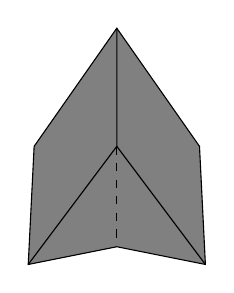
\begin{tikzpicture}[scale=.75]
		\draw[fill=gray] (0,0) -- (.1,2) -- (1.5,4) -- (2.9,2) -- (3,0) -- (1.5,.3) -- cycle;
		\draw (0,0) -- (1.5,2) -- (1.5,4);
		\draw (3,0) -- (1.5,2);
		\draw[dashed] (1.5,2) -- (1.5,.3);
	\end{tikzpicture}}
	
	Push the large triangular region inside
	&
	{\centering 
	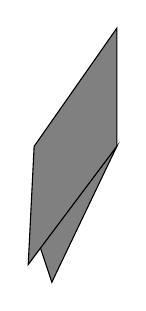
\begin{tikzpicture}[scale=.75]
		\draw[fill=gray] (1.5,2) -- (.4,-.3) -- (.2,.3) -- cycle;
		\draw[fill=gray] (0,0) -- (.1,2) -- (1.5,4) -- (1.5,2) -- cycle;
	\end{tikzpicture}}
	
	Flatten the parallelogram to complete the module.  Make seven more modules.
	&
	{\centering
	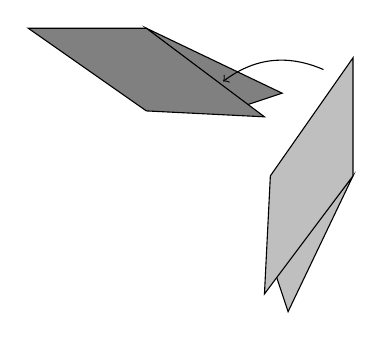
\begin{tikzpicture}[scale=.75]
		\begin{scope}[rotate=90]
					\draw[fill=gray] (1.5,2) -- (.4,-.3) -- (.2,.3) -- cycle;
		\draw[fill=gray] (0,0) -- (.1,2) -- (1.5,4) -- (1.5,2) -- cycle;
		\end{scope}
		\begin{scope}[xshift=0cm, yshift=-3cm]
					\draw[fill=lightgray] (1.5,2) -- (.4,-.3) -- (.2,.3) -- cycle;
		\draw[fill=lightgray] (0,0) -- (.1,2) -- (1.5,4) -- (1.5,2) -- cycle;
		\draw[->] (1,3.8) to[bend right] (-.7,3.6);
		\end{scope}
	\end{tikzpicture}}
	
	Insesrt one piece into another so that the folded edge of each module is on the outside
	\end{tabular}
	
	\begin{tabular}{p{2in}p{2in}p{2in}p{2in}}

	\centering
		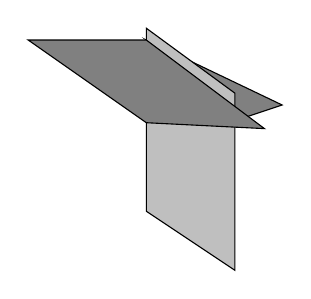
\begin{tikzpicture}[scale=.75]
		\begin{scope}[rotate=90]
					\draw[fill=gray] (1.5,2) -- (.4,-.3) -- (.2,.3) -- cycle;
% 		\draw[fill=gray] (0,0) -- (.1,2) -- (1.5,4) -- (1.5,2) -- cycle;
		\end{scope}
		\begin{scope}[xshift=-2cm, yshift=-1.4cm]
			\draw[fill=lightgray] (0,0) -- (0,3.1) -- (1.5,2) -- (1.5,-1) -- cycle;
		\end{scope}
		\begin{scope}[rotate=90]
				% 	\draw[fill=gray] (1.5,2) -- (.4,-.3) -- (.2,.3) -- cycle;
		\draw[fill=gray] (0,0) -- (.1,2) -- (1.5,4) -- (1.5,2) -- cycle;
		\end{scope}
		
	\end{tikzpicture}
	Be sure to tuck the inside piece as far into the fold as possible
	&
	\centering
		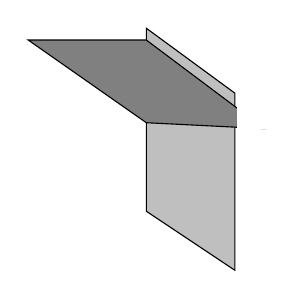
\begin{tikzpicture}[scale=.75]
		\begin{scope}[xshift=-2cm, yshift=-1.4cm]
			\draw[fill=lightgray] (0,0) -- (0,3.1) -- (1.5,2) -- (1.5,-1) -- cycle;
		\end{scope}
		\begin{scope}[rotate=90]
				% 	\draw[fill=gray] (1.5,2) -- (.4,-.3) -- (.2,.3) -- cycle;
		\draw[fill=gray] (0,0) -- (.1,2) -- (1.5,4) -- (1.5,2) -- cycle;
		\end{scope}
		\begin{scope}[yshift=0cm, xshift=-.45cm]
		    \draw[white, fill=white] (0,0) rectangle (.5,.5);
		\end{scope}
		
	\end{tikzpicture}
	Tuck the corners of the outside module into the grove of the inside module as snuggly as possible
	&
	{\centering
	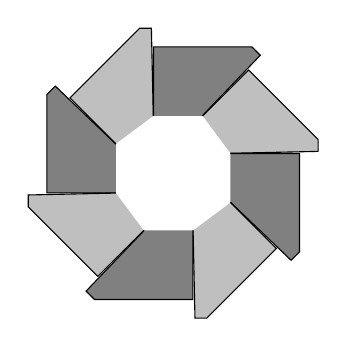
\begin{tikzpicture}[scale=.5]
	    \draw[white] (-1,0) node (A) {} -- ++(90:1) node (B) {} -- ++(45:1) node (C) {}-- ++(0:1) node (D) {}-- ++(-45:1) node (E) {}-- ++(-90:1) node (F) {}-- ++(-135:1) node (G) {}-- ++(-180:1) node (H) {}-- ++(-225:1) -- cycle ;
	    \draw[fill=gray] (A) -- ++(180:2) -- ++ (90:2.5)-- ++ (45:.3) -- (B) -- cycle ;
	    \draw[fill=lightgray] (B) -- ++(135:2) -- ++ (45:2.5)-- ++ (0:.3) -- (C) -- cycle ;
	    \draw[fill=gray] (C) -- ++(90:2) -- ++ (0:2.5)-- ++ (-45:.3) -- (D) -- cycle ;
	    \draw[fill=lightgray] (D) -- ++(45:2) -- ++ (-45:2.5)-- ++ (-90:.3) -- (E) -- cycle ;
	    \draw[fill=gray] (E) -- ++(0:2) -- ++ (-90:2.5)-- ++ (-135:.3) -- (F) -- cycle ;
	    \draw[fill=lightgray] (F) -- ++(-45:2) -- ++ (-135:2.5)-- ++ (-180:.3) -- (G) -- cycle ;
	    \draw[fill=gray] (G) -- ++(-90:2) -- ++ (-180:2.5)-- ++ (-225:.3) -- (H) -- cycle ;
	    \draw[fill=lightgray] (H) -- ++(-135:2) -- ++ (-225:2.5)-- ++ (-270:.3) -- (A) -- cycle ;
	\end{tikzpicture}}
	
	Continue to add modules around the octagon.  Tuck the corners of the last module on either side of the parallelogram inside the first module.
	&
	{\centering
	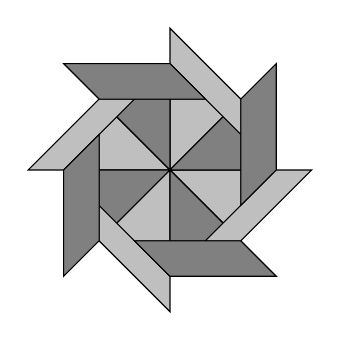
\begin{tikzpicture}[scale=.9]
	    \foreach \t in {90,0,-90,-180} {\draw[fill=lightgray] (0,0) -- ++(\t:1) -- ++ ({\t-90}:1) -- cycle; }
	    \foreach \t in {90,0,-90,-180} {\draw[fill=gray] (0,0) -- ++(\t:1) -- ++ ({\t+90}:1) -- cycle; }
	   	   \draw[fill=lightgray] (0,1.5) -- ++(0,.5) -- ++(1,-1) -- ++(0, -.5) -- cycle;
	   	   \draw[fill=lightgray] (1.5,0) -- ++(.5,0) -- ++(-1,-1) -- ++(-.5, 0) -- cycle;
	   	   \draw[fill=lightgray] (0,-1.5) -- ++(0,-.5) -- ++(-1,1) -- ++(0, .5) -- cycle;
	   	   \draw[fill=lightgray] (-1.5,0) -- ++(-.5,0) -- ++(1,1) -- ++(.5, 0) -- cycle;
	   	     \draw[fill=gray] (0,1.5) -- ++(.5,-.5) -- ++(-1.5,0) -- ++(-.5, .5) -- cycle;
	   	   \draw[fill=gray] (1.5,0) -- ++(-.5,-.5) -- ++(0,1.5) -- ++(.5, .5) -- cycle;
	   	   \draw[fill=gray] (0,-1.5) -- ++(-.5,.5) -- ++(1.5,0) -- ++(.5, -.5) -- cycle;
	   	   \draw[fill=gray] (-1.5,0) -- ++(.5,.5) -- ++(0,-1.5) -- ++(-.5, -.5) -- cycle;
	\end{tikzpicture}}
	
	Push gently to transform into a pinwheel.  If necessary, sharpen the creases and slide it in and out a few times.
\end{tabular} 

\end{landscape}